%%% lorem.tex --- 
%% 
%% Filename: lorem.tex
%% Description: 
%% Author: Ola Leifler
%% Maintainer: 
%% Created: Wed Nov 10 09:59:23 2010 (CET)
%% Version: $Id$
%% Version: 
%% Last-Updated: Wed Nov 10 09:59:47 2010 (CET)
%%           By: Ola Leifler
%%     Update #: 2
%% URL: 
%% Keywords: 
%% Compatibility: 
%% 
%%%%%%%%%%%%%%%%%%%%%%%%%%%%%%%%%%%%%%%%%%%%%%%%%%%%%%%%%%%%%%%%%%%%%%
%% 
%%% Commentary: 
%% 
%% 
%% 
%%%%%%%%%%%%%%%%%%%%%%%%%%%%%%%%%%%%%%%%%%%%%%%%%%%%%%%%%%%%%%%%%%%%%%
%% 
%%% Change log:
%% 
%% 
%% RCS $Log$
%%%%%%%%%%%%%%%%%%%%%%%%%%%%%%%%%%%%%%%%%%%%%%%%%%%%%%%%%%%%%%%%%%%%%%
%% 
%%% Code:






\chapter{Evaluation}
\label{cha:evaluation}

\section{Evaluation method}

The results of our anomaly detection techniques are first classified as True Positives (TP), True Negatives (TN), False Positives (FP) and False Negatives (FN) as shown in Table \ref{tab:anomaly_matrix}. With these classified data, we evaluate the techniques based on their precision:
$$ 
\text{Precision} = \frac{\text{TP}}{\text{TP} + \text{FP}} \quad \text{,}
$$
which captures how many of the predicted anomalies are actually true anomalies. A high precision means that fewer of the normal instances are incorrectly predicted as anomalies, and therefore reducing the FP rate. It is especially important in cases where FP wastes to much time and resources. With high precision, we ensure that the anomalies predicted by the anomaly detection technique are more likely to be real anomalies. To further understand the model's performance, we also evaluate the detection techniques based on their recall: 
$$
\text{Recall} = \frac{\text{TP}}{\text{TP} + \text{FN}} \quad \text{,}
$$
to evaluate how many true anomalies the model identifies. A high recall would mean that fewer actual anomalies are missed, which helps reduce the number of FN. If not missing an anomaly is of crucial importance, a high recall is very important to ensure that all potential issues are captured. Often, prioritizing recall and finding as many anomalies as possible comes at the cost of increasing FP. Finally, we also want to investigate the relationship between precision and recall. To evaluate this, we use \revrev{F1 score}{F1-score}, calculated as: 
$$
\text{F1-score} = 2 \times \frac{\text{Precision} \times \text{Recall}}{\text{Precision} + \text{Recall}} \quad \text{,}
$$
this metric is designed to balance the mean of precision and recall, and provides a single value that reflects the model's overall performance by balancing both precision and recall. The value gives us a good understanding of which technique is best when precision and recall are equally important. 

\begin{table}[t]
\centering
\fontspec{Roboto}
\begin{tabular}{|c|c|c|}
\hline
 & \textbf{Predicted Anomaly} & \textbf{Predicted Normal} \\
\hline
\textbf{Actual Anomaly} & True Positives (TP) & False Negatives (FN) \\
\hline
\textbf{Actual Normal} & False Positives (FP) & True Negatives (TN) \\
\hline
\end{tabular}
\caption{Matrix of Anomalies.}
\label{tab:anomaly_matrix}
\end{table}

\section{Results}
In this section the experimental results are provided. First, the results on each dataset are presented where all five algorithms are applied for both datasets. Then, results for offline and online anomaly detection are displayed. In all tests, the goal is to achieve the highest possible F1-score.

\subsection{HDFS} 
The results of the anomaly detectors when applied on the HDFS dataset are shown in Figure~\ref{fig:hdfs-v1-results}. The results shown are precision, recall and F1- score for \revrev{}{SVM}, Isolation Forest, PCA, LogClustering, Half-Space Trees and One-Class SVM. \revrev{}{SVM, serving as a benchmark for the other algorithms, demonstrates high results.} LogClustering showed the best results \revrev{}{out of the unsupervised methods }in all three evaluation metrics. PCA also demonstrates good results, providing the second best results in all three evaluation parameters. Isolation Forest exhibits relative consistent performance, with precision, recall, and F1-score values remaining closely aligned. Half-Space Trees provides a high precision, but a low recall resulting at an F1-score of $33$\%. One-Class SVM shows the weakest results out of all algorithms, however the results are fairly stable. For each algorithm, precision yields the highest score, whereas recall consistently results in the lowest.

\begin{figure}[t]
    \centering
    {\fontspec{Roboto}
    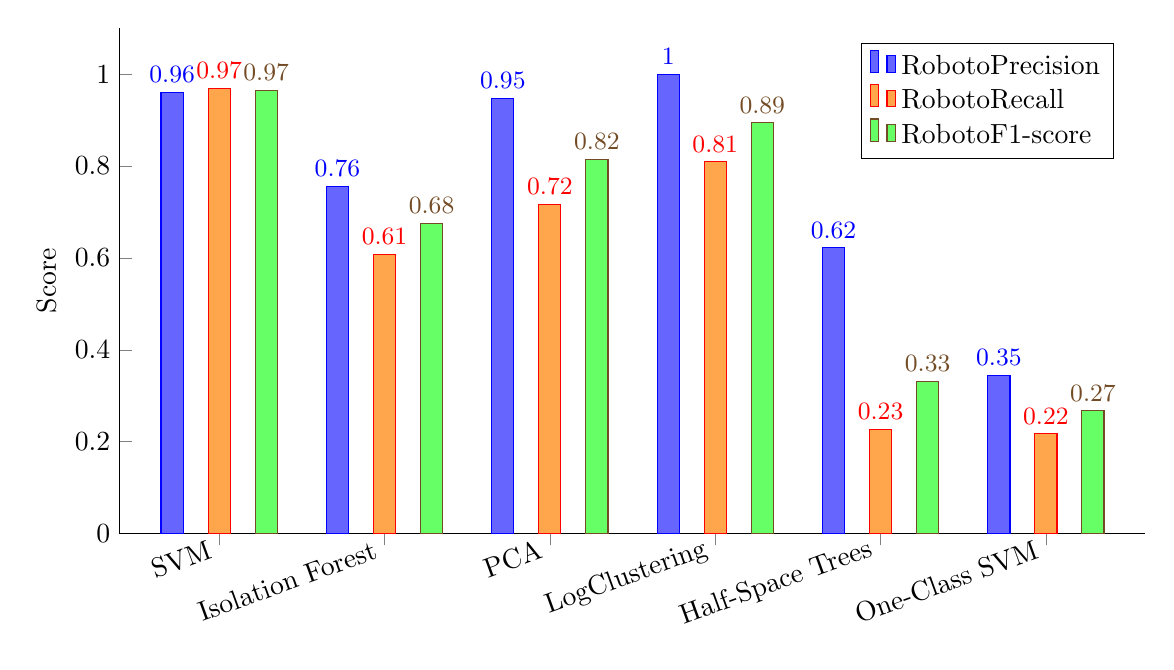
\begin{tikzpicture}
        \begin{axis}[
            ybar,
            bar width=8pt,
            x=2.1cm,
            width=14cm,
            height=8cm,
            enlarge x limits=0.12,
            ylabel={Score},
            symbolic x coords={SVM, Isolation Forest, PCA, LogClustering, Half-Space Trees, One-Class SVM},
            xtick=data,
            xticklabel style={rotate=20, anchor=east},
            legend style={at={(0.97,0.97)}, anchor=north east, font = \fontspec{Roboto}},
            legend cell align=left,
            ymin=0, ymax=1.1,
            nodes near coords,
            nodes near coords align={vertical},
            every node near coord/.append style={font=\small},
            ylabel near ticks,
            axis x line*=bottom,
            axis y line*=left
        ]
        %Precision
        \addplot+[style={fill=blue!60}, bar shift=-17pt] coordinates {
           (SVM, 0.961)
            (Isolation Forest, 0.756)
            (PCA, 0.947)
            (LogClustering, 1.000)
            (Half-Space Trees, 0.622)
            (One-Class SVM, 0.345)
        };
        %Recall
        \addplot+[style={fill=orange!70}, bar shift=0pt] coordinates {
            (SVM, 0.969)
            (Isolation Forest, 0.608)
            (PCA, 0.716)
            (LogClustering, 0.809)
            (Half-Space Trees, 0.227)
            (One-Class SVM, 0.217)
        };
        %F1
        \addplot+[style={fill=green!60}, bar shift=17pt] coordinates {
        (SVM, 0.965)
            (Isolation Forest, 0.675)
            (PCA, 0.815)
            (LogClustering, 0.894)
            (Half-Space Trees, 0.332)
            (One-Class SVM, 0.267)
        };
        \legend{Precision, Recall, F1-score}
        \end{axis}
    \end{tikzpicture}
    }
    \caption[Comparison of anomaly detection techniques on HDFS dataset]{Comparison of anomaly detection techniques on HDFS dataset \revrev{}{(results rounded to two decimal places)}.}
    \label{fig:hdfs-v1-results}
\end{figure}

\subsection{BGL}

This section provides the results of each algorithm evaluated on the BGL dataset. Since a sliding window approach was applied, different window sizes and step sizes were explored. The corresponding results for these are also shown. The evaluated window sizes are 4, 6, and 8 hours, each paired with step sizes of 1, 2, and 3 hours, respectively.

\revrev{}{\subsubsection{SVM}
The results shown in Figure \ref{fig:svm_all_metrics} indicate very similar performance across the different window and step sizes. Precision remains consistently at 100\%, while recall varies more. The highest recall is achieved with a window size of 8 and a step size of 3. This slightly higher recall results in the best F1-score, reaching 99.8\%.
}

\begin{figure}[t]
    \centering
    % Shared legend at the very top, centered:
    \makebox[\textwidth]{\ref{sharedlegend}}
    \vspace{0.5cm} % Space between legend and subfigures
    % Subfigure 1 - Precision
    \begin{subfigure}[t]{0.31\textwidth}
        \centering
        {\fontspec{Roboto}
        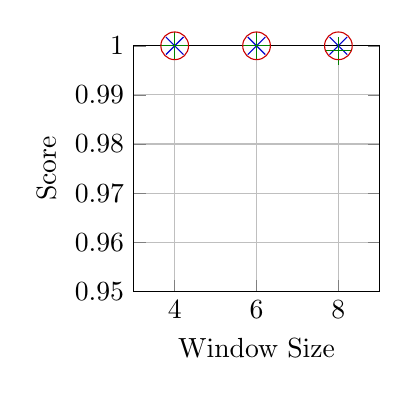
\begin{tikzpicture}
            \begin{axis}[
                xlabel={Window Size},
                ylabel={Score},
                xmin=3, xmax=9,
                ymin=0.95, ymax=1,
                xtick={4,6,8},
                ytick={0.95,0.96,0.97,0.98,0.99,1},
                width=4.7cm,
                height=4.7cm,
                grid=both,
                scatter/classes={
    step1={mark=x, mark size=4.5pt, draw=blue!80!black},
    step2={mark=+, mark size=5pt, draw=green!50!black},
    step3={mark=o, mark size=5pt, fill=red!50, draw=red!80!black}
},
                legend style={draw=none},
            ]
            \addplot[scatter, only marks, scatter src=explicit symbolic]
            coordinates {
                (4,1) [step1] 
                (6,1) [step1]
                (8,1) [step1]
                (4,1) [step2]
                (6,1) [step2]
                (8,0.999) [step2]
                (4,1) [step3]
                (6,1) [step3]
                (8,1) [step3]
            };
            \end{axis}
        \end{tikzpicture}
        }
        \vspace*{-0.43cm}
        \caption{\fontspec{Roboto} Precision}
    \end{subfigure}%
    \hspace{0.01\textwidth}%
    % Subfigure 2 - Recall
    \begin{subfigure}[t]{0.31\textwidth}
        \centering
        {\fontspec{Roboto}
        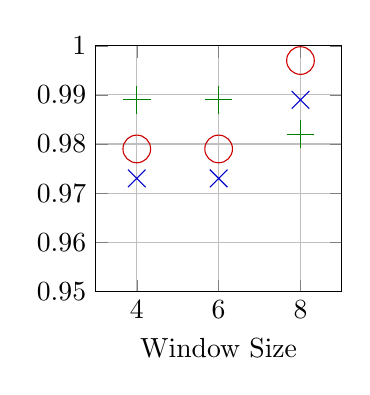
\begin{tikzpicture}
            \begin{axis}[
                xlabel={Window Size},
                xmin=3, xmax=9,
                ymin=0.95, ymax=1,
                xtick={4,6,8},
                ytick={0.95,0.96,0.97,0.98,0.99,1},
                width=4.7cm,
                height=4.7cm,
                grid=both,
                scatter/classes={
                      step1={mark=x, mark size=4.5pt, draw=blue!80!black},
    step2={mark=+, mark size=5pt, draw=green!50!black},
    step3={mark=o, mark size=5pt, fill=red!50, draw=red!80!black}
                },
                legend style={draw=none},
            ]
            \addplot[scatter, only marks, scatter src=explicit symbolic]
            coordinates {
                (4,0.973) [step1]
                (6,0.973) [step1]
                (8,0.989) [step1]
                (4,0.989) [step2]
                (6,0.989) [step2]
                (8,0.982) [step2]
                (4,0.979) [step3]
                (6,0.979) [step3]
                (8,0.997) [step3]
            };
            \end{axis}
        \end{tikzpicture}
        }
        \caption{\fontspec{Roboto} Recall}
    \end{subfigure}%
    \hspace{0.01\textwidth}%
    % Subfigure 3 - F1-Score
    \begin{subfigure}[t]{0.31\textwidth}
        \centering
        {\fontspec{Roboto}
        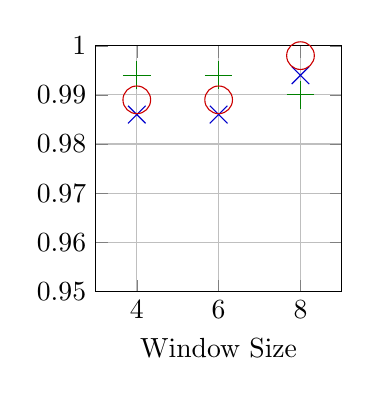
\begin{tikzpicture}
            \begin{axis}[
                xlabel={Window Size},
                xmin=3, xmax=9,
                ymin=0.95, ymax=1,
                xtick={4,6,8},
                ytick={0.95,0.96,0.97,0.98,0.99,1},
                width=4.7cm,
                height=4.7cm,
                grid=both,
                scatter/classes={
                      step1={mark=x, mark size=4.5pt, draw=blue!80!black},
                      step2={mark=+, mark size=5pt, draw=green!50!black},
                      step3={mark=o, mark size=5pt, fill=red!50, draw=red!80!black}},
                legend to name=sharedlegend,
                legend style={font = \fontspec{Roboto},draw=black, legend columns=3},
            ]
            \addplot[scatter, only marks, scatter src=explicit symbolic]
            coordinates {
                (4,0.986) [step1]
                (6,0.986) [step1]
                (8,0.994) [step1]
                (4,0.994) [step2]
                (6,0.994) [step2]
                (8,0.990) [step2]
                (4,0.989) [step3]
                (6,0.989) [step3]
                (8,0.998) [step3]
            };
            \legend{Step Size = 1, Step Size = 2, Step Size = 3}
            \end{axis}
        \end{tikzpicture}
        }
        \caption{\fontspec{Roboto} F1-score}
    \end{subfigure}

    \vspace{0.7cm}

    \caption{\revrev{}{Impact of window size and step size using SVM on the BGL dataset.}}
    \label{fig:svm_all_metrics}

    \vspace{0.5cm}
    \centering
  

\end{figure}

\subsubsection{Isolation Forest}
As seen in Figure \ref{fig:if_all_metrics} the window size has a big impact on all three evaluation metrics. Further, the step size has less impact, slightly affecting the results of each window size. For the three evaluated window sizes, precision, recall and F1-score exhibits similar trends. Notably, a window size of 6 hours consistently shows the weakest results, while a window size of 8 hours shows the highest results across all three metrics. The results consistently show that a window size of 4 and 8 hours performs best when paired with a step size of 3 hours, while window size of 6 hours performs best when paired with a step size of 1 hour. 

\begin{figure}[t]
    \centering
    % Shared legend at the very top, centered:
    \makebox[\textwidth]{\ref{sharedlegend}}
    \vspace{0.5cm} % Space between legend and subfigures
    % Subfigure 1 - Precision
    \begin{subfigure}[t]{0.31\textwidth}
        \centering
        {\fontspec{Roboto}
        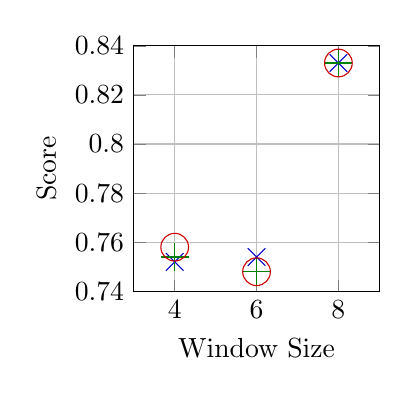
\begin{tikzpicture}
            \begin{axis}[
                xlabel={Window Size},
                ylabel={Score},
                xmin=3, xmax=9,
                ymin=0.74, ymax=0.84,
                xtick={4,6,8},
                ytick={0.74,0.76,0.78,0.80,0.82,0.84},
                width=4.7cm,
                height=4.7cm,
                grid=both,
                scatter/classes={
    step1={mark=x, mark size=4.5pt, draw=blue!80!black},
    step2={mark=+, mark size=5pt, draw=green!50!black},
    step3={mark=o, mark size=5pt, fill=red!50, draw=red!80!black}
},
                legend style={draw=none},
            ]
            \addplot[scatter, only marks, scatter src=explicit symbolic]
            coordinates {
                (4,0.752) [step1]
                (6,0.754) [step1]
                (8,0.833) [step1]
                (4,0.754) [step2]
                (6,0.748) [step2]
                (8,0.833) [step2]
                (4,0.758) [step3]
                (6,0.748) [step3]
                (8,0.833) [step3]
            };
            \end{axis}
        \end{tikzpicture}
        }
        \vspace*{-0.43cm}
        \caption{\fontspec{Roboto} Precision}
    \end{subfigure}%
    \hspace{0.01\textwidth}%
    % Subfigure 2 - Recall
    \begin{subfigure}[t]{0.31\textwidth}
        \centering
        {\fontspec{Roboto}
        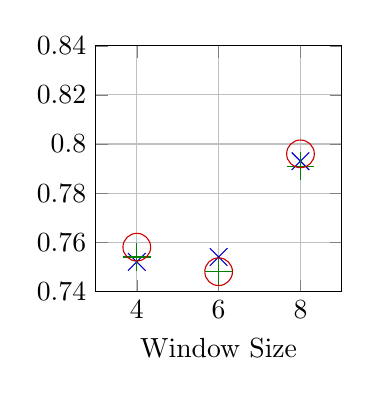
\begin{tikzpicture}
            \begin{axis}[
                xlabel={Window Size},
                xmin=3, xmax=9,
                ymin=0.74, ymax=0.84,
                xtick={4,6,8},
                ytick={0.74,0.76,0.78,0.80,0.82,0.84},
                width=4.7cm,
                height=4.7cm,
                grid=both,
                scatter/classes={
                      step1={mark=x, mark size=4.5pt, draw=blue!80!black},
    step2={mark=+, mark size=5pt, draw=green!50!black},
    step3={mark=o, mark size=5pt, fill=red!50, draw=red!80!black}
                },
                legend style={draw=none},
            ]
            \addplot[scatter, only marks, scatter src=explicit symbolic]
            coordinates {
                (4,0.752) [step1]
                (6,0.754) [step1]
                (8,0.793) [step1]
                (4,0.754) [step2]
                (6,0.748) [step2]
                (8,0.791) [step2]
                (4,0.758) [step3]
                (6,0.748) [step3]
                (8,0.796) [step3]
            };
            \end{axis}
        \end{tikzpicture}
        }
        \caption{\fontspec{Roboto} Recall}
    \end{subfigure}%
    \hspace{0.01\textwidth}%
    % Subfigure 3 - F1-Score
    \begin{subfigure}[t]{0.31\textwidth}
        \centering
        {\fontspec{Roboto}
        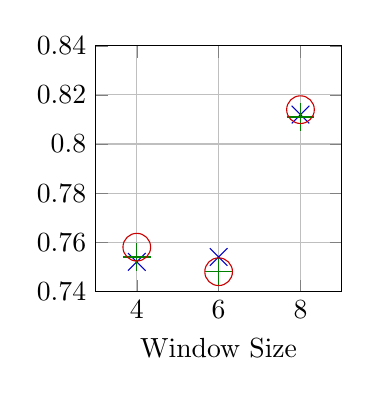
\begin{tikzpicture}
            \begin{axis}[
                xlabel={Window Size},
                xmin=3, xmax=9,
                ymin=0.74, ymax=0.84,
                xtick={4,6,8},
                ytick={0.74,0.76,0.78,0.80,0.82,0.84},
                width=4.7cm,
                height=4.7cm,
                grid=both,
                scatter/classes={
                      step1={mark=x, mark size=4.5pt, draw=blue!80!black},
                      step2={mark=+, mark size=5pt, draw=green!50!black},
                      step3={mark=o, mark size=5pt, fill=red!50, draw=red!80!black}},
                legend to name=sharedlegend,
                legend style={font = \fontspec{Roboto},draw=black, legend columns=3},
            ]
            \addplot[scatter, only marks, scatter src=explicit symbolic]
            coordinates {
                (4,0.752) [step1]
                (6,0.754) [step1]
                (8,0.812) [step1]
                (4,0.754) [step2]
                (6,0.748) [step2]
                (8,0.811) [step2]
                (4,0.758) [step3]
                (6,0.748) [step3]
                (8,0.814) [step3]
            };
            \legend{Step Size = 1, Step Size = 2, Step Size = 3}
            \end{axis}
        \end{tikzpicture}
        }
        \caption{\fontspec{Roboto} F1-score}
    \end{subfigure}

    \vspace{0.7cm}

    \caption{Impact of window size and step size using Isolation Forest on the BGL dataset.}
    \label{fig:if_all_metrics}

    \vspace{0.5cm}
    \centering
  

\end{figure}



\subsubsection{PCA}
The results for PCA are presented in Figure \ref{fig:pca_all_metrics}, where the precision is shown to be significantly higher when using an 8 hours window size. The recall results also show the best results when using an 8 hour window size, however the 4 hour window size exhibits the weakest recall, closely aligned to the results of the 6 hour window size. The F1-score is also the highest for the 8 hour window size, while the 4 and 6 hour window size show similar results, and the 2 hour step size gives the best results for all 3 window sizes. Once again, the step size has a minimal affect on the results for the three metrics, and the window size of 8 consistently outperformed the other configurations across all three metrics. 



\begin{figure}[t]
    \centering
    % Shared legend at the very top, centered:
    \makebox[\textwidth]{\ref{sharedlegend}}
    \vspace{0.5cm} % Space between legend and subfigures
    % Subfigure 1 - Precision
    \begin{subfigure}[t]{0.31\textwidth}
        \centering
        {\fontspec{Roboto}
        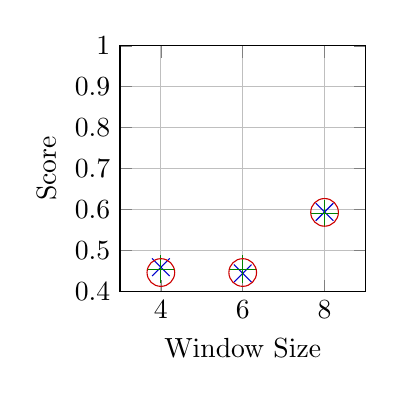
\begin{tikzpicture}
            \begin{axis}[
                xlabel={Window Size},
                ylabel={Score},
                xmin=3, xmax=9,
                ymin=0.4, ymax=1,
                xtick={4,6,8},
                ytick={0.4, 0.5, 0.6, 0.7, 0.8, 0.9, 1.0},
                width=4.7cm,
                height=4.7cm,
                grid=both,
                scatter/classes={
    step1={mark=x, mark size=4.5pt, draw=blue!80!black},
    step2={mark=+, mark size=5pt, draw=green!50!black},
    step3={mark=o, mark size=5pt, fill=red!50, draw=red!80!black}
},
                legend style={draw=none},
            ]
            \addplot[scatter, only marks, scatter src=explicit symbolic]
            coordinates {
               (4,0.459) [step1]
            (6,0.444) [step1]
            (8,0.594) [step1]
            (4,0.454) [step2]
            (6,0.454) [step2]
            (8,0.590) [step2]
            (4,0.446) [step3]
            (6,0.446) [step3]
            (8,0.593) [step3]
            };
            \end{axis}
        \end{tikzpicture}
        }
        \vspace*{-0.43cm}
        \caption{\fontspec{Roboto} Precision}
        \label{precisionPCABGL}
    \end{subfigure}%
    \hspace{0.01\textwidth}%
    % Subfigure 2 - Recall
    \begin{subfigure}[t]{0.31\textwidth}
        \centering
        {\fontspec{Roboto}
        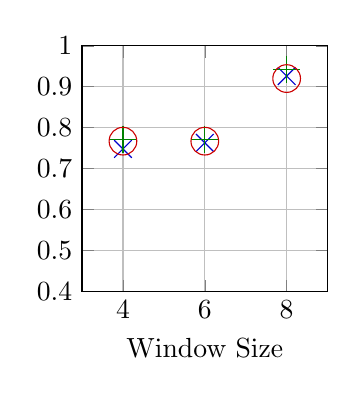
\begin{tikzpicture}
            \begin{axis}[
                xlabel={Window Size},
                xmin=3, xmax=9,
               ymin=0.4, ymax=1,
                xtick={4,6,8},
                ytick={0.4, 0.5, 0.6, 0.7, 0.8, 0.9,1.0},
                width=4.7cm,
                height=4.7cm,
                grid=both,
                scatter/classes={
                      step1={mark=x, mark size=4.5pt, draw=blue!80!black},
    step2={mark=+, mark size=5pt, draw=green!50!black},
    step3={mark=o, mark size=5pt, fill=red!50, draw=red!80!black}
                },
                legend style={draw=none},
            ]
            \addplot[scatter, only marks, scatter src=explicit symbolic]
            coordinates {
                (4,0.748) [step1]
            (6,0.763) [step1]
            (8,0.926) [step1]
            (4,0.771) [step2]
            (6,0.771) [step2]
            (8,0.942) [step2]
            (4,0.767) [step3]
            (6,0.767) [step3]
            (8,0.920) [step3]
            };
            \end{axis}
        \end{tikzpicture}
        }
        \caption{\fontspec{Roboto} Recall}
        \label{recallPCABGL}
    \end{subfigure}%
    \hspace{0.01\textwidth}%
    % Subfigure 3 - F1-Score
    \begin{subfigure}[t]{0.31\textwidth}
        \centering
        {\fontspec{Roboto}
        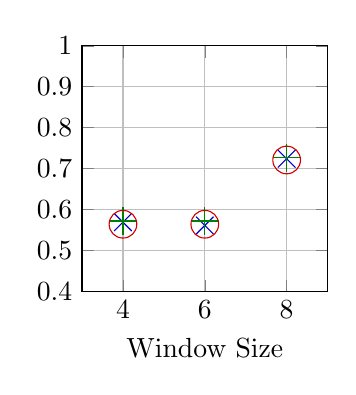
\begin{tikzpicture}
            \begin{axis}[
                xlabel={Window Size},
                xmin=3, xmax=9,
                ymin=0.4, ymax=1,
                xtick={4,6,8},
                ytick={0.4, 0.5, 0.6, 0.7, 0.8, 0.9,1.0},
                width=4.7cm,
                height=4.7cm,
                grid=both,
                scatter/classes={
                      step1={mark=x, mark size=4.5pt, draw=blue!80!black},
                      step2={mark=+, mark size=5pt, draw=green!50!black},
                      step3={mark=o, mark size=5pt, fill=red!50, draw=red!80!black}},
                legend to name=sharedlegend,
                legend style={font= \fontspec{Roboto},draw=black, legend columns=3},
            ]
            \addplot[scatter, only marks, scatter src=explicit symbolic]
            coordinates {
                (4,0.569) [step1]
            (6,0.561) [step1]
            (8,0.724) [step1]
            (4,0.572) [step2]
            (6,0.572) [step2]
            (8,0.726) [step2]
            (4,0.564) [step3]
            (6,0.564) [step3]
            (8,0.721) [step3]
            };
            \legend{Step Size = 1, Step Size = 2, Step Size = 3}
            \end{axis}
        \end{tikzpicture}
        
        }
        \caption{\fontspec{Roboto} F1-score}
    \end{subfigure}

    \vspace{0.7cm}

    \caption{Impact of window size and step size using PCA on the BGL dataset.}
    \label{fig:pca_all_metrics}
    \vspace{0.5cm}
    \centering
  

\end{figure}
\subsubsection{LogClustering}
The results for when LogClustering is applied on the BGL dataset are presented in Figure \ref{fig:logclustering_all_metrics}. Once again, it is evident that the 8-hour window size produces the best results. However, the step size has a more significant impact on the outcomes than previously, showing more noticeable variations in performance. Step size of 3 hours performs best when studying F1-score and recall, but a 2 hours step size provides the best results for precision. 


\begin{figure}[t]
    \centering
    % Shared legend at the very top, centered:
    \makebox[\textwidth]{\ref{sharedlegend}}
    \vspace{0.5cm} % Space between legend and subfigures
    % Subfigure 1 - Precision
    \begin{subfigure}[t]{0.31\textwidth}
        \centering
        {\fontspec{Roboto}
        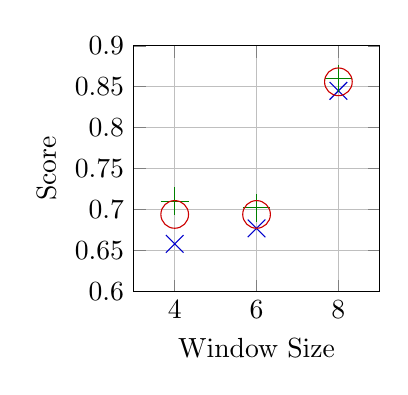
\begin{tikzpicture}
            \begin{axis}[
                xlabel={Window Size},
                ylabel={Score},
                xmin=3, xmax=9,
                ymin=0.6, ymax=0.9,
                xtick={4,6,8},
                ytick={0.60, 0.65, 0.70, 0.75, 0.80, 0.85, 0.90},
                width=4.7cm,
                height=4.7cm,
                grid=both,
                scatter/classes={
    step1={mark=x, mark size=4.5pt, draw=blue!80!black},
    step2={mark=+, mark size=5pt, draw=green!50!black},
    step3={mark=o, mark size=5pt, fill=red!50, draw=red!80!black}
},
                legend style={draw=none},
            ]
            \addplot[scatter, only marks, scatter src=explicit symbolic]
            coordinates {
                (4,0.658) [step1]
            (6,0.677) [step1]
            (8,0.845) [step1]
            (4,0.710) [step2]
            (6,0.702) [step2]
            (8,0.860) [step2]
            (4,0.694) [step3]
            (6,0.694) [step3]
            (8,0.856) [step3]
            };
            \end{axis}
        \end{tikzpicture}
        }
        \vspace*{-0.43cm}
        \caption{\fontspec{Roboto} Precision}
    \end{subfigure}%
    \hspace{0.01\textwidth}%
    % Subfigure 2 - Recall
    \begin{subfigure}[t]{0.31\textwidth}
        \centering
        {\fontspec{Roboto}
        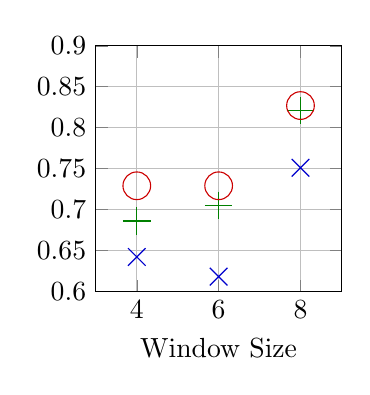
\begin{tikzpicture}
            \begin{axis}[
                xlabel={Window Size},
                xmin=3, xmax=9,
                ymin=0.6, ymax=0.9,
                xtick={4,6,8},
                ytick={0.60, 0.65, 0.70, 0.75, 0.80, 0.85, 0.90},
                width=4.7cm,
                height=4.7cm,
                grid=both,
                scatter/classes={
                      step1={mark=x, mark size=4.5pt, draw=blue!80!black},
    step2={mark=+, mark size=5pt, draw=green!50!black},
    step3={mark=o, mark size=5pt, fill=red!50, draw=red!80!black}
                },
                legend style={draw=none},
            ]
            \addplot[scatter, only marks, scatter src=explicit symbolic]
            coordinates {
                (4,0.642) [step1]
            (6,0.618) [step1]
            (8,0.751) [step1]
            (4,0.686) [step2]
            (6,0.705) [step2]
            (8,0.821) [step2]
            (4,0.729) [step3]
            (6,0.729) [step3]
            (8,0.827) [step3]
            };
            \end{axis}
        \end{tikzpicture}
        }
        \caption{\fontspec{Roboto} Recall}
    \end{subfigure}%
    \hspace{0.01\textwidth}%
    % Subfigure 3 - F1-Score
    \begin{subfigure}[t]{0.31\textwidth}
        \centering
        {\fontspec{Roboto}
        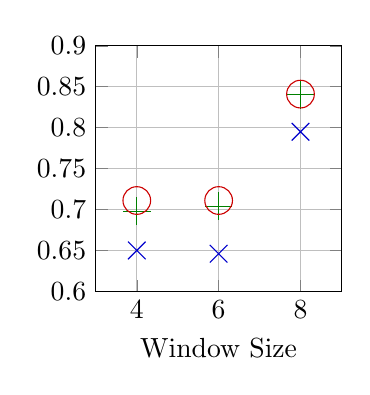
\begin{tikzpicture}
            \begin{axis}[
                xlabel={Window Size},
                xmin=3, xmax=9,
                ymin=0.6, ymax=0.9,
                xtick={4,6,8},
                ytick={0.60, 0.65, 0.70, 0.75, 0.80, 0.85, 0.90},
                width=4.7cm,
                height=4.7cm,
                grid=both,
                scatter/classes={
                      step1={mark=x, mark size=4.5pt, draw=blue!80!black},
                      step2={mark=+, mark size=5pt, draw=green!50!black},
                      step3={mark=o, mark size=5pt, fill=red!50, draw=red!80!black}},
                legend to name=sharedlegend,
                legend style={font=\fontspec{Roboto},draw=black, legend columns=3},
            ]
            \addplot[scatter, only marks, scatter src=explicit symbolic]
            coordinates {
                (4,0.650) [step1]
            (6,0.646) [step1]
            (8,0.795) [step1]
            (4,0.698) [step2]
            (6,0.704) [step2]
            (8,0.840) [step2]
            (4,0.711) [step3]
            (6,0.711) [step3]
            (8,0.841) [step3]
            };
            \legend{Step Size = 1, Step Size = 2, Step Size = 3}
            \end{axis}
        \end{tikzpicture}
        }
        \caption{\fontspec{Roboto} F1-score}
    \end{subfigure}

    \vspace{0.7cm}

    \caption{Impact of window size and step size using LogClustering on the BGL dataset.}
    \label{fig:logclustering_all_metrics}

    \vspace{0.5cm}
    \centering
  

\end{figure}





\subsubsection{Overall results for BGL}
Based on the tested window and step sizes, we selected the one with the best F1-score to represent the specific algorithm. The results of all algorithms when applied to the BGL datasets are shown in Figure \ref{fig:bgl-results}. \revrev{}{The benchmark algorithm SVM obtains the F1-score of 99.8\%. Studying the unsupervised methods,} LogClustering provides the best \revrev{F1 score}{F1-score}, demonstrates exceptional consistency across all three metrics. Isolation Forest also shows a stable result, with performance just below LogClustering. PCA provides the highest recall, but fairly weak results when studying the F1-score and precision. Studying the online methods results, One-Class SVM performs slightly better than HST on the BGL dataset, with a high recall. The BGL dataset contains significantly more unique log events compared to HDFS, resulting in a greater number of event combinations and a wider variety of anomalies. One-Class SVM can handle this better because of its use of continuous feature space, making it better at detecting hidden anomalies.

\begin{figure}[t]
    \centering
    {\fontspec{Roboto}
    \begin{tikzpicture}
        \begin{axis}[
            ybar,
            bar width=8pt,
            x=2.1cm,
            width=14cm,
            height=8cm,
            enlarge x limits=0.12,
            ylabel={Score},
            symbolic x coords={SVM, Isolation Forest, PCA, LogClustering, Half-Space Trees, One-Class SVM},
            xtick=data,
            xticklabel style={rotate=20, anchor=east},
            legend style={at={(0.97,0.97)}, anchor=north east, \fontspec{Roboto}},
            legend cell align=left,
            ymin=0, ymax=1.1,
            nodes near coords,
            nodes near coords align={vertical},
            every node near coord/.append style={font=\small},
            ylabel near ticks,
            axis x line*=bottom,
            axis y line*=left
        ]
        % Precision
        \addplot+[style={fill=blue!60}, bar shift=-17pt] coordinates {
            (SVM, 1)
            (Isolation Forest, 0.833) %window=8, step=3
            (PCA, 0.590) %window=8, step=2
            (LogClustering, 0.856) %window=8, step=3
            (Half-Space Trees, 0.143)
            (One-Class SVM, 0.1693)
        };
        % Recall
        \addplot+[style={fill=orange!70}, bar shift=0pt] coordinates {
            (SVM, 0.997)
            (Isolation Forest, 0.796) %window=8, step=3
            (PCA, 0.942) %window=8, step=2
            (LogClustering, 0.827) %window=8, step=3
            (Half-Space Trees, 0.358)
            (One-Class SVM, 0.5799)
        };
        % F1-score
        \addplot+[style={fill=green!60}, bar shift=17pt] coordinates {
        (SVM, 0.998)
            (Isolation Forest, 0.814) %window=8, step=3
            (PCA, 0.726) %window=8, step=2
            (LogClustering, 0.841) %window=8, step=3
            (Half-Space Trees, 0.205)
            (One-Class SVM, 0.2621)
        };
        \legend{Precision, Recall, F1-score}
        \end{axis}
    \end{tikzpicture}
    }
    \caption[Comparison of anomaly detection techniques on BGL dataset]{Comparison of anomaly detection techniques on BGL dataset \revrev{}{(results rounded to two decimal places)}.}
    \label{fig:bgl-results}
\end{figure}

\subsection{Offline vs Online}
This section presents the results for both offline and online algorithms when applied on the two datasets. In Figure \ref{fig:offline-vs-online-combined} the performance of the algorithms is averaged within each group by calculating the mean value \revrev{}{of the unsupervised algorithms (SVM excluded)}.


\begin{figure}[t]
    \centering
    {\fontspec{Roboto}
    % Shared legend
    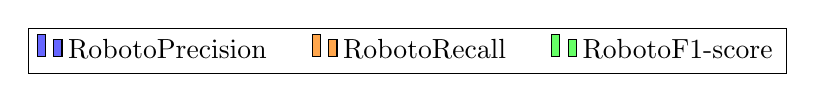
\begin{tikzpicture}
        \begin{axis}[
            hide axis,
            xmin=0, xmax=1,
            ymin=0, ymax=1,
            legend columns=3,
            legend style={
                at={(0.5,1.05)},
                anchor=south,
                draw=black,
                font=\fontspec{Roboto},
                /tikz/every even column/.append style={column sep=0.5cm}
            },
        ]
        \addlegendimage{ybar, ybar legend, fill=blue!60}
        \addlegendimage{ybar, ybar legend, fill=orange!70}
        \addlegendimage{ybar, ybar legend, fill=green!60}
        \addlegendentry{Precision}
        \addlegendentry{Recall}
        \addlegendentry{F1-score}
        \end{axis}
    \end{tikzpicture}

    % Subfigures
    \begin{subfigure}[t]{0.49\textwidth}
        \centering
       
        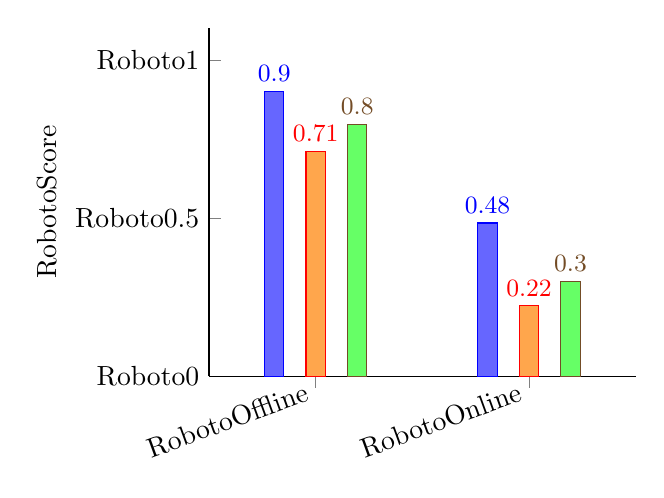
\begin{tikzpicture}
            \begin{axis}[
                font=\fontspec{Roboto},
                ybar,
                bar width=7pt,
                width=7cm,
                height=6cm,
                enlarge x limits=0.50,
                ylabel={Score},
                symbolic x coords={Offline, Online},
                xtick=data,
                xticklabel style={rotate=20, anchor=east},
                ymin=0, ymax=1.1,
                nodes near coords,
                nodes near coords align={vertical},
                every node near coord/.append style={font=\small},
                ylabel near ticks,
                axis x line*=bottom,
                axis y line*=left
            ]
            \addplot+[style={fill=blue!60}, bar shift=-15pt] coordinates {
                (Offline, 0.901)  
                (Online, 0.484) 
            };
            \addplot+[style={fill=orange!70}, bar shift=0pt] coordinates {
                (Offline, 0.711) 
                (Online, 0.222) 
            };
            \addplot+[style={fill=green!60}, bar shift=15pt] coordinates {
                (Offline, 0.795)
                (Online, 0.30)
            };
            \end{axis}
        \end{tikzpicture}
        \caption{\fontspec{Roboto} HDFS}
        \label{fig:HDFS-offline-vs-online-results}
    \end{subfigure}
    \hfill
    \begin{subfigure}[t]{0.49\textwidth}
       
        \centering
        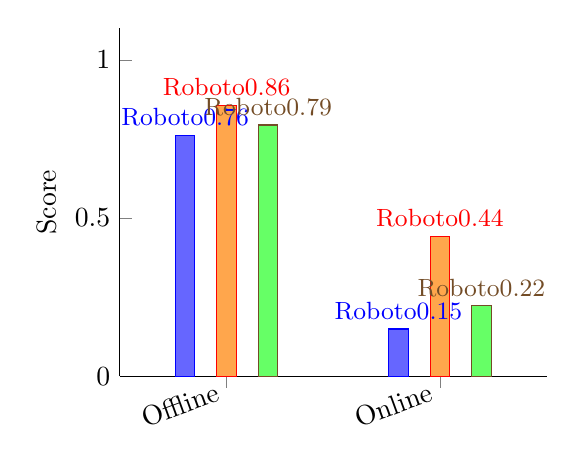
\begin{tikzpicture}
            \begin{axis}[
                ybar,
                bar width=7pt,
                width=7cm,
                height=6cm,
                enlarge x limits=0.50,
                ylabel={Score},
                symbolic x coords={Offline, Online},
                xtick=data,
                xticklabel style={rotate=20, anchor=east},
                ymin=0, ymax=1.1,
                nodes near coords,
                nodes near coords align={vertical},
                every node near coord/.append style={font=\small\fontspec{Roboto}},
                ylabel near ticks,
                axis x line*=bottom,
                axis y line*=left
            ]
            \addplot+[style={fill=blue!60}, bar shift=-15pt] coordinates {
                (Offline, 0.760)  
                (Online, 0.149) 
            };
            \addplot+[style={fill=orange!70}, bar shift=0pt] coordinates {
                (Offline, 0.855) 
                (Online, 0.442) 
            };
            \addplot+[style={fill=green!60}, bar shift=15pt] coordinates {
                (Offline, 0.794)
                (Online, 0.222)
            };
            \end{axis}
        \end{tikzpicture}
        \caption{\fontspec{Roboto} BGL}
        \label{fig:BGL-offline-vs-online-results}
    \end{subfigure}
    \caption[Offline vs Online performance on HDFS and BGL datasets]{Offline vs Online performance on HDFS and BGL datasets \revrev{}{(results rounded to two decimal places)}.}
    \label{fig:offline-vs-online-combined}
    }
\end{figure}

\subsubsection{HDFS}
As shown in Figure \ref{fig:HDFS-offline-vs-online-results}, the offline algorithms Isolation Forest, PCA and LogClustering perform much better than the online techniques Half-Space Trees and One-Class SVM on average. The offline methods result in a mean of $80$\% in F1-score, whereas the online algorithms only provide a mean of $30$\%. Notably, online methods produce significantly higher precision compared to recall. Offline techniques, on the other hand, maintain a more balanced relationship between precision and recall, despite a difference of $19$ percentage points. Offline methods are likely more stable due to the fact that they hold full access to the datasets during training. This enables them to capture underlying distribution, and model both normal and anomalous behavior better. The online methods instead operate incrementally with limited context, making them more conservative while also having more trouble to detect diverse anomaly patterns. This often leads to a lower recall, causing less stability for the online methods. 


\subsubsection{BGL}
For the BGL dataset, offline methods significantly outperform online techniques. As shown in Figure \ref{fig:BGL-offline-vs-online-results}, offline algorithms achieve an average F1-score of $79$\%, whereas online algorithms record a substantially lower F1-score of just $22$\%. In particular, online methods produce significantly higher recall compared to precision. Offline techniques, on the other hand, achieve a more balanced relationship between recall and precision.


\section{Summary of results}
The experimental results show that LogClustering performs the best on both datasets. When the algorithms are applied to the HDFS dataset, all algorithms show precision as its strongest metric. This does not go for the BGL dataset however, where the values are either close to each other or recall shows the highest value. Additionally, offline anomaly detectors outperform online anomaly detectors, delivering just above twice the performance across all three evaluation metrics. Among the online methods, Half-Space Trees achieved the best performance on the HDFS dataset, while One-Class SVM recorded the best results on the BGL dataset.

%%%%%%%%%%%%%%%%%%%%%%%%%%%%%%%%%%%%%%%%%%%%%%%%%%%%%%%%%%%%%%%%%%%%%%
%%% lorem.tex ends here

%%% Local Variables: 
%%% mode: latex
%%% TeX-master: "demothesis"
%%% End: 
